% ============================================================
%  Chapter 6 — Illuminating Problems
%  Nature-Inspired Optimisation for Delivery Problems (2022)
%  Self-contained Beamer slides (reader-friendly, no presenter needed)
% ============================================================
\documentclass[aspectratio=169,10pt]{beamer}

\usetheme{Madrid}
\usecolortheme{seahorse}

\usepackage{amsmath,amssymb}
\usepackage{graphicx}
\usepackage{booktabs}
\usepackage{array}
\usepackage{listings}
\usepackage{xcolor}
\usepackage{tikz}
\usepackage{hyperref}
\usepackage{microtype}

\graphicspath{{figures/}}

% ── listings style ──────────────────────────────────────────
\lstset{
  language=Java,
  basicstyle=\ttfamily\scriptsize,
  numbers=left,
  numberstyle=\tiny\color{gray},
  frame=single,
  backgroundcolor=\color{gray!7},
  keywordstyle=\color{blue!70!black}\bfseries,
  commentstyle=\color{green!50!black}\itshape,
  stringstyle=\color{orange!80!black},
  breaklines=true,
  showstringspaces=false,
  tabsize=2,
  captionpos=b,
}

\lstdefinestyle{python}{
  language=Python,
  basicstyle=\ttfamily\scriptsize,
  numbers=left,
  numberstyle=\tiny\color{gray},
  frame=single,
  backgroundcolor=\color{gray!7},
  keywordstyle=\color{blue!70!black}\bfseries,
  commentstyle=\color{green!50!black}\itshape,
  stringstyle=\color{orange!80!black},
  breaklines=true,
  showstringspaces=false,
  tabsize=2,
}

% ── footer ──────────────────────────────────────────────────
\setbeamertemplate{footline}[frame number]
\setbeamertemplate{navigation symbols}{}

% ── title ───────────────────────────────────────────────────
\title[Chapter 6 — Illuminating Problems]{%
  \textbf{Chapter 6: Illuminating Problems}\\
  \large Quality-Diversity and MAP-Elites for Delivery Planning}
\subtitle{Nature-Inspired Optimisation for Delivery Problems (2022)}
\author{Lecture notes based on the book}
\date{2022}

% ============================================================
\begin{document}
% ============================================================

\begin{frame}
  \titlepage
\end{frame}

% ────────────────────────────────────────────────────────────
\begin{frame}[allowframebreaks]{Chapter Overview}
% ────────────────────────────────────────────────────────────

This chapter introduces a fundamentally different philosophy for
optimisation: rather than searching for \emph{one} best solution,
the goal is to produce a \emph{rich map} of many high-quality
solutions that span the entire space of possible outcomes.
This idea is called \textbf{illumination}, and the central algorithm
is called \textbf{MAP-Elites}.

\medskip
\begin{block}{Why illumination matters for delivery planning}
In logistics, a single ``optimal'' solution may become unusable
overnight if a vehicle breaks down, staff call in sick, or a last-minute
change of plan is required.
Rather than re-running a lengthy optimisation from scratch, a manager
who has an \emph{archive} of diverse, high-quality plans can simply
pick the plan that best fits today's constraints---in seconds, not hours.
The on-demand economy, where customers expect near-instant delivery,
makes this capability increasingly critical.
\end{block}

\medskip
\textbf{Chapter road-map}:
\begin{itemize}
  \item \textbf{6.1 Introduction} --- quality-diversity algorithms and
        the case for illumination.
  \item \textbf{6.2 Illumination Algorithms --- MAP-Elites} --- the
        behaviour space, niches (bins), and the archive data structure.
  \item \textbf{6.3 Using MAP-Elites to Plan Deliveries} --- applying
        MAP-Elites to a multi-mode supermarket delivery problem with
        nine solution characteristics.
  \item \textbf{6.4 Results} --- archive coverage, solution diversity,
        and interactive filtering via constraints and aspirations.
  \item \textbf{6.5 Conclusions} --- when illumination pays off, and
        design choices that matter.
\end{itemize}

\end{frame}

% ============================================================
\section{6.1 Introduction: Quality-Diversity}
% ============================================================

\begin{frame}[allowframebreaks]{6.1 Introduction: The Case for Diversity}

Classical optimisation returns a single answer.
Multi-objective optimisation returns a \emph{Pareto front}---a set of
solutions where no one objective can be improved without worsening
another.
\textbf{Quality-Diversity (QD)} algorithms go further: they seek a
\emph{structured collection} of high-quality solutions that covers as
much of the behaviour space as possible.

\medskip
\begin{block}{Definition: Quality-Diversity Algorithm}
A Quality-Diversity algorithm is an evolutionary algorithm that
simultaneously optimises for (1) \emph{quality} (each solution in
the collection must be as fit as possible within its region) and
(2) \emph{diversity} (the collection must represent as many distinct
regions of the solution space as possible).
\end{block}

\medskip
\begin{figure}
  \centering
  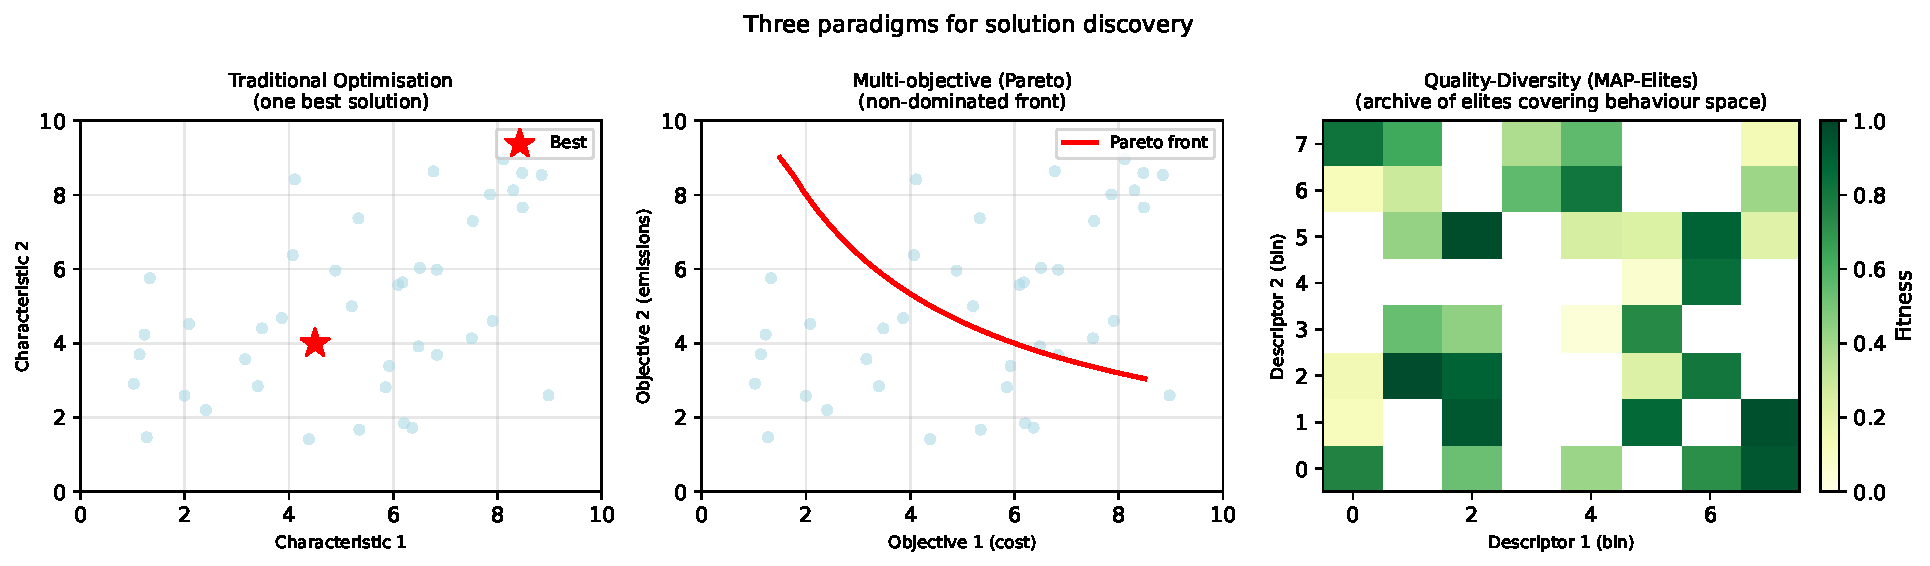
\includegraphics[width=0.88\linewidth]{fig_qd_concept.pdf}
  \caption{Three paradigms for solution discovery.
           Traditional optimisation returns one best point.
           Multi-objective optimisation returns a Pareto front.
           Quality-Diversity fills an archive grid with the best
           solution found for \emph{every} region of the space.}
\end{figure}

\framebreak

\textbf{The delivery planning context.}
Consider a supermarket that must plan daily routes for its vans and
cargo bikes.
The planner cares about many things simultaneously:
total cost, staff cost, emissions, the fraction of deliveries made
by bike, how many vehicles are needed, and so on.
A traditional single-objective algorithm might minimise total cost,
but the resulting plan might be environmentally unacceptable.
A bi-objective algorithm could trade cost against emissions, but it
ignores the other seven concerns.

MAP-Elites, the illumination algorithm studied in this chapter,
produces an archive of hundreds or thousands of plans, each one
the best solution ever found for a particular combination of
cost-level and emission-level (and other characteristics).
The planner can then \emph{browse} this archive and select the plan
that matches today's operational priorities---without waiting for a
new optimisation run.

\medskip
\begin{alertblock}{Key Insight: Illumination shifts decision-making}
Traditional algorithms make decisions \emph{inside} the optimiser
(``which objective do I weight most?'').
Illumination algorithms shift this decision \emph{outside} to the
human expert, who can apply domain knowledge \emph{after} the
archive has been built.
This is especially valuable when priorities change frequently---as they
do in on-demand logistics.
\end{alertblock}

\end{frame}

% ============================================================
\section{6.2 Illumination Algorithms: MAP-Elites}
% ============================================================

\begin{frame}[allowframebreaks]{6.2 MAP-Elites: Core Idea}

MAP-Elites stands for \textbf{Map Archive of Phenotypic Elites}.
It was introduced by Mouret and Clune (2015) in the paper
\emph{Illuminating Search Spaces by Mapping Elites}.
The central idea is to maintain a structured map (or grid) of
solutions, where each \emph{cell} in the grid holds the single best
solution ever discovered for that particular region of the
\textbf{behaviour space}.

\medskip
\begin{block}{Definition: Behaviour Space and Behaviour Descriptors}
The \textbf{behaviour space} is a multi-dimensional space whose axes
are \emph{solution characteristics}---measurable properties of a
solution that describe \emph{how} it behaves, rather than how good
it is.
Examples: the total financial cost $c$, the CO$_2$ emissions $e$,
the fraction of deliveries made by cargo bike.
A \textbf{behaviour descriptor} is a specific choice of such
characteristics used to define the axes of the archive grid.
\end{block}

\medskip
\textbf{A concrete example.}
Suppose a logistics problem has two solution characteristics:
financial cost $c$ and environmental impact (CO$_2$ emissions) $e$.
Imagine we evolved the following four solutions:

\medskip
\begin{center}
\begin{tabular}{cc}
\toprule
$c$ (cost) & $e$ (emissions) \\
\midrule
500 & 1023 \\
550 & 1050 \\
610 &  990 \\
490 & 1120 \\
\bottomrule
\end{tabular}
\end{center}

\framebreak

\begin{figure}
  \centering
  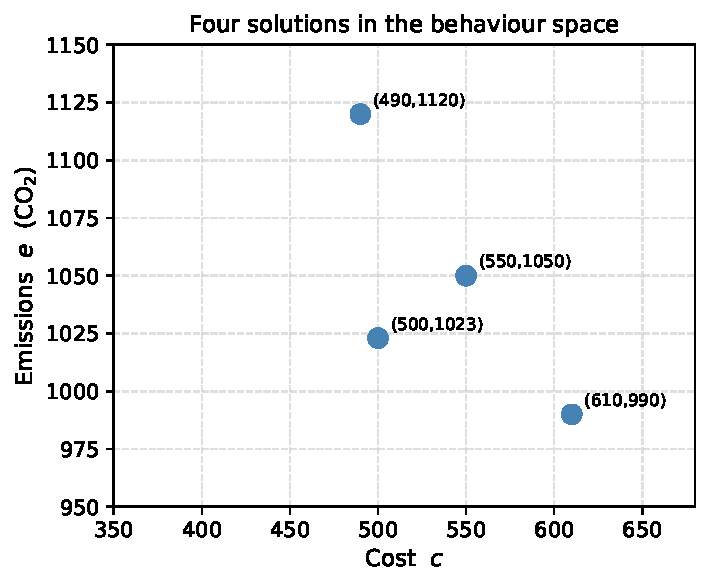
\includegraphics[width=0.55\linewidth]{fig_solution_scatter.pdf}
  \caption{The four solutions plotted in the two-dimensional behaviour
           space ($c$ on the horizontal axis, $e$ on the vertical axis).
           Each point represents one complete delivery plan.}
\end{figure}

Because both $c$ and $e$ are integers with $c \in [350, 650]$ and
$e \in [950, 1140]$, there are theoretically
$(650 - 350) \times (1140 - 950) = 300 \times 190 = 57{,}000$
possible $(c,e)$ pairs.
Storing 57,000 solutions is impractical:
(1) the memory overhead could be enormous;
(2) many combinations may not correspond to any valid plan;
(3) many solutions may be nearly identical;
(4) many may be of poor quality.

MAP-Elites solves this by \textbf{scaling} the raw characteristics into
a much smaller grid.
For example, with $b = 20$ bins per axis, we obtain an archive of only
$20 \times 20 = 400$ cells.

\end{frame}

% ────────────────────────────────────────────────────────────
\begin{frame}[allowframebreaks]{6.2 MAP-Elites: The Bin-Scaling Formula}
% ────────────────────────────────────────────────────────────

To place a solution into the archive, each raw characteristic value
$r$ must be translated into a \textbf{scaled bin index} $s$.
The following three-step formula performs this translation.

\medskip
\begin{block}{Bin-Scaling Formula}
Let $r$ be the raw value of one characteristic, let $min$ and $max$
be the known minimum and maximum values of that characteristic, and
let $b$ be the number of bins per axis.
Then:
\[
  \delta = (max + 1) - min
\]
\[
  cap = \frac{\delta}{b}
\]
\[
  s = \mathrm{int}\!\left(\frac{r - min}{cap} + 1\right)
\]
\end{block}

\begin{block}{Notation}
\begin{itemize}
  \item $\delta$ (delta) is the \emph{total range} of the
        characteristic (number of distinct integer values it can take).
        Adding 1 ensures the maximum value maps to bin $b$ rather than
        falling outside.
  \item $cap$ (capacity) is the \emph{width} of each bin---how many
        raw values fall into each cell.
  \item $b$ is the number of bins per dimension (e.g., $b=20$).
  \item $s$ is the resulting bin index (from 1 to $b$).
        The function $\mathrm{int}(\cdot)$ truncates to the nearest
        integer below (floor).
\end{itemize}
\end{block}

\framebreak

\begin{alertblock}{How to Read the Scaling Formula}
The formula maps any value in $[min, max]$ uniformly onto $\{1, 2,
\ldots, b\}$.
The larger $r$ is, the larger $s$ is---the relationship is linear.
If we double $b$ (use finer bins), $cap$ halves and the archive becomes
more detailed but sparser (fewer solutions per cell on average).
Choosing $b$ is a design trade-off: large $b$ gives fine resolution
but requires more evaluations to fill the archive; small $b$ fills
quickly but loses detail.
\end{alertblock}

\medskip
\begin{figure}
  \centering
  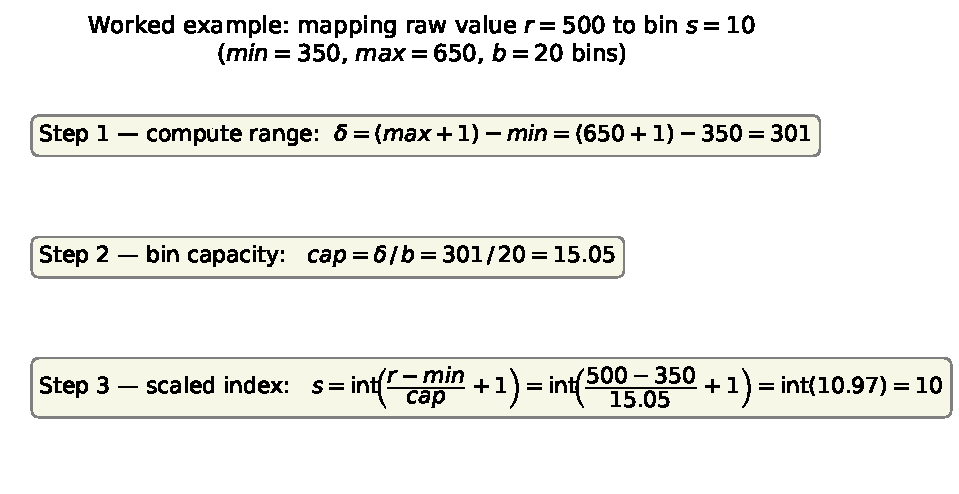
\includegraphics[width=0.75\linewidth]{fig_scaling_formula.pdf}
  \caption{Worked example: the raw cost value $r = 500$ with
           $min = 350$, $max = 650$, and $b = 20$ bins maps to
           scaled bin index $s = 10$.}
\end{figure}

\framebreak

\textbf{Worked example for all four solutions.}
Using $c \in [350, 650]$ and $e \in [950, 1140]$, with $b = 20$:

\medskip
\begin{center}
\renewcommand{\arraystretch}{1.2}
\begin{tabular}{cccc}
\toprule
\multicolumn{2}{c}{Raw values} & \multicolumn{2}{c}{Bin index} \\
\cmidrule(lr){1-2}\cmidrule(lr){3-4}
$c$ & $e$ & $s_c$ & $s_e$ \\
\midrule
500 & 1023 & 10 &  8 \\
550 & 1050 & 14 & 11 \\
610 &  990 & 18 &  5 \\
490 & 1120 & 10 & 18 \\
\bottomrule
\end{tabular}
\end{center}

\medskip
The four solutions occupy four different cells in the 20$\times$20
archive grid:

\medskip
\begin{columns}
\begin{column}{0.45\textwidth}
  \begin{figure}
    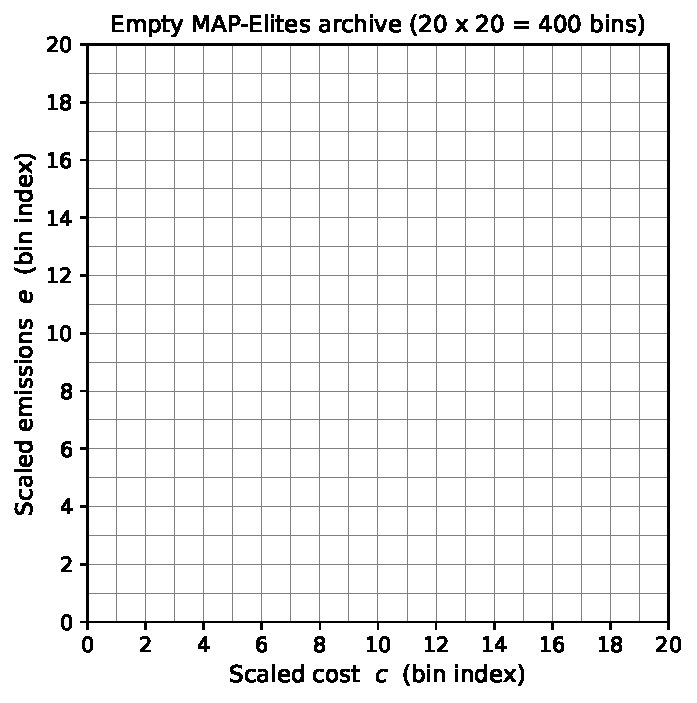
\includegraphics[width=\linewidth]{fig_archive_empty.pdf}
    \caption{The empty 400-cell archive, ready to receive solutions.}
  \end{figure}
\end{column}
\begin{column}{0.45\textwidth}
  \begin{figure}
    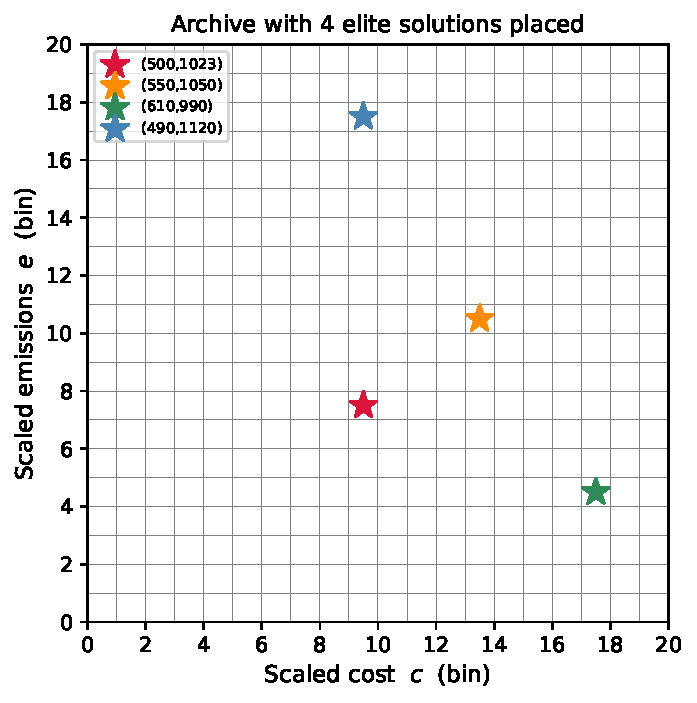
\includegraphics[width=\linewidth]{fig_archive_filled.pdf}
    \caption{After placing the four solutions: each star marks one
             occupied cell.  396 cells remain empty.}
  \end{figure}
\end{column}
\end{columns}

\end{frame}

% ────────────────────────────────────────────────────────────
\begin{frame}[allowframebreaks]{6.2 MAP-Elites: The Fitness Value and Archive Update}
% ────────────────────────────────────────────────────────────

The behaviour descriptors tell us \emph{which cell} a solution belongs
to.
But two different solutions can map to the same cell.
To decide which solution gets to occupy a cell, MAP-Elites uses a
\textbf{fitness value} $f$.

\medskip
\begin{block}{Fitness in MAP-Elites}
The fitness value $f$ measures the \emph{quality} of a solution,
independently of its behaviour descriptors.
In the delivery problem, $f$ could be the total distance travelled:
shorter routes are better (lower $f$).
The archive update rule is: ``a new solution $n$ replaces the current
occupant of a cell only if $f(n) < f(\text{current})$\,''.
This ensures every cell always holds the \emph{best} solution found
so far for that region of the behaviour space.
\end{block}

\medskip
\textbf{Intuition.}
Think of each cell as a mini-competition.
Two solutions with the same (cost-level, emissions-level) combination
compete directly: whichever has the lower total distance wins the cell.
Solutions in different cells do not compete---they represent genuinely
different trade-offs.

\medskip
\begin{exampleblock}{Worked Example: Cell Collision}
Suppose cell $(10, 8)$ is already occupied by a solution with
$c=500$, $e=1023$, total distance $f=340$\,km.
A new solution arrives with $c=512$, $e=1020$, total distance
$f=330$\,km.
Both map to cell $(10, 8)$ (same bin indices under our scaling).
Since $330 < 340$, the new solution \emph{replaces} the old one.
The archive now holds a slightly better solution in that cell.
\end{exampleblock}

\framebreak

\begin{alertblock}{Key Insight: Decoupling quality from diversity}
In MAP-Elites, quality (fitness) and diversity (cell location) are
\emph{decoupled}.
The fitness function evaluates quality \emph{within} a cell.
The behaviour descriptors decide \emph{which} cell.
This is fundamentally different from a Pareto approach, where the same
objectives serve both purposes simultaneously.
The decoupling gives the algorithm designer much more flexibility in
choosing what counts as ``good'' vs.\ what counts as ``different''.
\end{alertblock}

\end{frame}

% ────────────────────────────────────────────────────────────
\begin{frame}[allowframebreaks]{6.2 MAP-Elites: The Algorithm (Algorithm 14)}
% ────────────────────────────────────────────────────────────

The MAP-Elites algorithm is conceptually simple: initialise with
random solutions, then repeatedly generate new candidates (by
recombination or mutation), evaluate them, and attempt to add them
to the archive.
The algorithm continues until a total-evaluations budget
\texttt{totEvals} is exhausted.

\medskip
\begin{block}{Algorithm 14: MAP-Elites (pseudocode)}
\begin{enumerate}
  \item Set $buckets = 20$, $dimensions = 2$, $evals = 0$.
  \item Initialise the map (archive).
  \item \textbf{Initialisation phase:} while $evals < init$:
    \begin{enumerate}
      \item $n \leftarrow$ \texttt{newIndividual()} \quad (random solution)
      \item $evals \mathrel{+}= 1$
      \item \texttt{add(map, n)}
    \end{enumerate}
  \item \textbf{Main loop:} while $evals < totEvals$:
    \begin{enumerate}
      \item If \texttt{random()} $<$ \texttt{xoverPressure}: \\
            $c \leftarrow$ \texttt{newIndividual(map.random(), map.random())}
            \quad (crossover two random parents from archive)
      \item Else: \\
            $c \leftarrow$ \texttt{newIndividual(map.random())}
            \quad (clone one random parent)
      \item $c$.\texttt{mutate()} \quad (always apply mutation)
      \item \texttt{add(map, c)}
    \end{enumerate}
  \item Return the archive.
\end{enumerate}
\end{block}

\framebreak

\textbf{The \texttt{add} procedure.}
Adding a solution to the archive requires just three steps:
\begin{enumerate}
  \item Compute the \emph{key} (bin index tuple) for the solution: \\
        $key \leftarrow$ \texttt{getKey(n)} \quad
        (apply the bin-scaling formula to each characteristic)
  \item If \texttt{map.get(key) == null}: the cell is empty, so place
        the solution directly: \texttt{map.put(key, n)}.
  \item Else: the cell is occupied.
        Let $old = $ \texttt{map.get(key)}.
        If \texttt{new.fitness() < old.fitness()}: replace the
        occupant: \texttt{map.put(key, n)}.
\end{enumerate}

\medskip
\begin{figure}
  \centering
  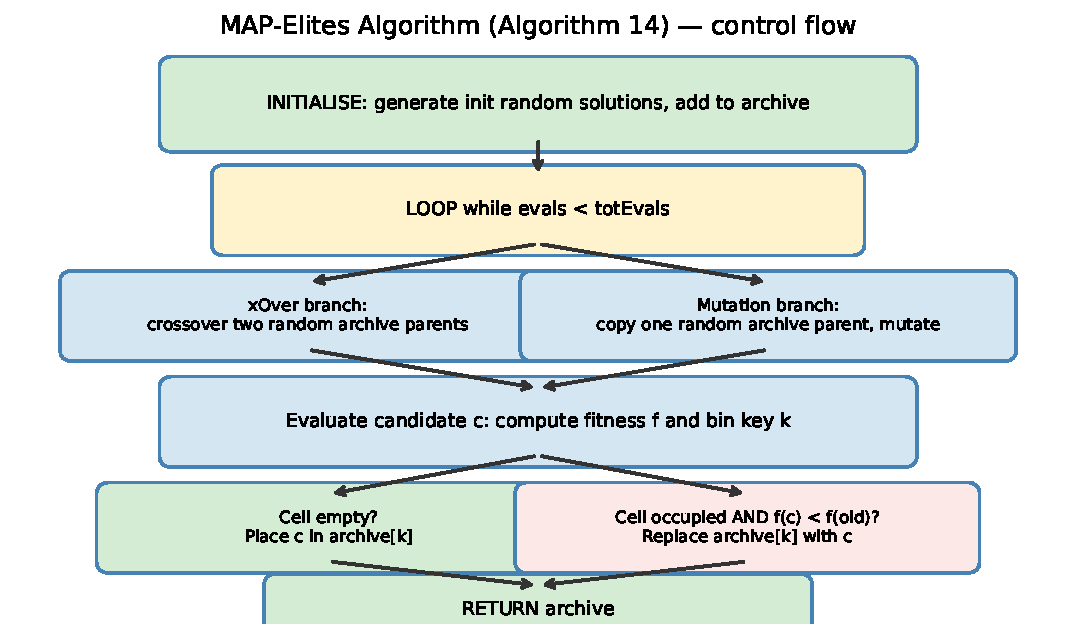
\includegraphics[width=0.75\linewidth]{fig_map_elites_flow.pdf}
  \caption{Control flow of the MAP-Elites algorithm.
           After initialisation, the main loop alternates between
           generating candidates (crossover or clone+mutate) and
           attempting to add them to the archive.}
\end{figure}

\framebreak

\textbf{Two key design parameters.}

\textbf{(1) xOverPressure} controls the fraction of candidates
generated by crossover versus mutation.
A value of 0.5 means crossover and mutation are equally likely.
Higher values bias the search towards combining existing archive
solutions; lower values rely more on random mutation.

\textbf{(2) totEvals} (total evaluations) is the computational budget.
Each call to evaluate a candidate costs one evaluation.
More evaluations generally means a fuller, higher-quality archive,
but also more computation time.

\medskip
\begin{alertblock}{Key Insight: The archive as both population and result}
In a standard evolutionary algorithm, the population holds candidate
solutions during the search and is discarded at the end.
In MAP-Elites, the archive \emph{is} the population \emph{and} the
final result.
At every point during the run, the archive is a complete, usable
set of diverse elite solutions.
The algorithm never ``loses'' diversity by replacing the whole
population---once a cell is filled, that solution is preserved
until something strictly better comes along.
\end{alertblock}

\end{frame}

% ────────────────────────────────────────────────────────────
\begin{frame}[allowframebreaks]{6.2 Archive Capacity and Sparse Storage}
% ────────────────────────────────────────────────────────────

With $b$ bins per dimension and $d$ dimensions, the archive has a
theoretical capacity of:

\medskip
\begin{block}{Archive Capacity Formula}
\[
  c = b^d
\]
where $c$ is the total number of cells, $b$ (the bucket count) is
the number of bins per dimension (axis), and $d$ is the number of
dimensions (solution characteristics used as behaviour descriptors).
For $b = 20$ and $d = 2$: $c = 20^2 = 400$.
For $b = 10$ and $d = 9$: $c = 10^9 = 1{,}000{,}000{,}000$.
\end{block}

\medskip
\begin{alertblock}{How to Read This: Exponential growth}
The capacity grows \emph{exponentially} with the number of dimensions.
Doubling the number of dimensions squares the capacity.
This is the famous ``\textbf{curse of dimensionality}'': adding even
one more behaviour descriptor multiplies the required archive storage
by $b$.
For $b = 10$, going from 8 to 9 dimensions multiplies the archive
by 10, from $10^8$ to $10^9$ cells.
\end{alertblock}

\medskip
In practice, for the FabFoods/supermarket delivery problem with
9 characteristics and $b = 10$, the theoretical archive size is $10^9$.
Creating a Java array of $10^9$ slots would exhaust JVM heap memory.
The solution is a \textbf{sparse map (dictionary)}: instead of
pre-allocating all cells, the archive is stored as a hash map that
only allocates memory for \emph{occupied} cells.
As solutions are found, new entries are added on demand.
This way a sparse archive of 500 occupied cells uses only 500 entries,
not $10^9$.

\medskip
The cells are identified by \textbf{keys}: arrays of integers, one
value per dimension, each value being the scaled bin index of the
solution's characteristic.
For example, the key $[10, 8]$ identifies the cell at scaled-cost
bin 10, scaled-emissions bin 8.

\end{frame}

% ============================================================
\section{6.3 Using MAP-Elites to Plan Deliveries}
% ============================================================

\begin{frame}[allowframebreaks]{6.3 The Delivery Planning Problem}
% ────────────────────────────────────────────────────────────

The scenario studied in this chapter extends the supermarket delivery
problem introduced in Chapter 5.
The supermarket now operates a \textbf{mixed fleet}: conventional vans
\emph{and} cargo bikes.
A new delivery plan must be generated for each working day, because
the number of deliveries and their locations change with customer
demand.

\medskip
\begin{block}{Problem: Multi-Mode Supermarket Delivery}
Given a set of customers with delivery time windows and quantity
requirements, and a depot, plan routes for vans and cargo bikes such
that:
\begin{itemize}
  \item every customer is served within their time window;
  \item vehicle capacity constraints are respected;
  \item a rich archive of diverse, high-quality plans is produced,
        covering the full range of cost/emissions/bike-usage trade-offs.
\end{itemize}
\end{block}

\medskip
\textbf{Why add cargo bikes?}
Cargo bikes produce zero CO$_2$ emissions and have low running costs,
making them attractive for sustainability-conscious businesses.
However, they have much smaller capacity and lower speed than vans.
Depending on the day's delivery profile, the optimal mix of vans
and bikes will vary.
MAP-Elites builds an archive that shows the manager the full range
of van/bike combinations and their associated costs and emissions,
so that the manager---not the algorithm---decides how green to be
on any given day.

\end{frame}

% ────────────────────────────────────────────────────────────
\begin{frame}[allowframebreaks]{6.3 The Cost Model (Table 6.2)}
% ────────────────────────────────────────────────────────────

A \textbf{cost model} is needed to evaluate solutions realistically.
The model assigns costs based on the vehicles used, the distance
travelled, the time taken, and the number of reload trips.
The variables and values used in this chapter are shown below.

\medskip
\begin{block}{Delivery Cost Model (Table 6.2)}
\begin{center}
\renewcommand{\arraystretch}{1.25}
\begin{tabular}{lccc}
\toprule
Parameter & Van & Cargo Bike \\
\midrule
Capacity (units) & 100 & 20 \\
Fixed cost per day (\pounds) & 164 & 16 \\
Running cost per km (\pounds) & 0.117 & 0.010 \\
Staff cost per hour (\pounds) & 12 & 12 \\
Loading time between runs (min) & 30 & 15 \\
Speed (km/h) & 10 & 1 \\
Emissions (g CO$_2$/km) & 158 & 0 \\
\bottomrule
\end{tabular}
\end{center}
\end{block}

\medskip
\begin{block}{Notation and Meaning}
\begin{itemize}
  \item \textbf{Fixed cost per day}: paid regardless of how much the
        vehicle is used.
        A van parked all day still costs \pounds164; a bike costs
        \pounds16.
  \item \textbf{Running cost per km}: fuel/maintenance cost proportional
        to distance driven.
        A van costs about 12$\times$ more per km than a bike to run.
  \item \textbf{Staff cost per hour}: the same for both modes (\pounds12),
        because a human operator rides both.
  \item \textbf{Loading time}: the time between completing one run and
        starting the next (reload + dispatch).
        Vans take 30 minutes to reload; bikes take 15 minutes.
  \item \textbf{Speed}: vans are 10$\times$ faster than bikes
        (10 km/h vs.\ 1 km/h), which dramatically affects how many
        customers a bike can serve per day.
  \item \textbf{Emissions}: vans emit 158\,g CO$_2$/km; bikes emit zero.
\end{itemize}
\end{block}

\framebreak

\begin{alertblock}{How to Read the Cost Model}
These numbers reveal a fundamental trade-off: bikes are \emph{much}
cheaper to run and produce zero emissions, but they are 10$\times$
slower and carry only one-fifth the capacity of a van.
A bike that takes 5 hours to complete one delivery run (at 1 km/h,
covering perhaps 5 km) might do the same work as a van in 30 minutes.
The time difference translates directly into \emph{staff cost}, which
is the dominant cost for slow vehicles.
The optimal vehicle mix therefore depends on the spatial distribution
and quantities of today's deliveries.
\end{alertblock}

\medskip
\textbf{Nine solution characteristics} (behaviour descriptors) are
tracked for each solution (Table 6.1):
\begin{enumerate}
  \item Total daily fixed cost
  \item Total staff cost
  \item Total vehicle running cost
  \item Cost per delivery (per unit crate)
  \item Emissions produced (g CO$_2$)
  \item Percentage of deliveries made by bike
  \item Percentage of distance covered by bike
  \item Number of bicycles required
  \item Number of vans required
\end{enumerate}

These nine characteristics form the axes of the MAP-Elites archive.
With $b = 10$ bins per axis, the archive has $10^9$ possible cells,
stored sparsely as described earlier.

\end{frame}

% ────────────────────────────────────────────────────────────
\begin{frame}[allowframebreaks]{6.3 Solution Characteristics (Table 6.1)}
% ────────────────────────────────────────────────────────────

The nine characteristics serve two roles simultaneously: they are
\textbf{behaviour descriptors} (they define the cell in the archive)
and \textbf{decision criteria} (the manager uses them to choose a plan).
This dual role is one of the key design insights in this chapter.

\medskip
\begin{block}{Why nine characteristics?}
A traditional bi-objective formulation would pick two objectives and
trade them off.
But real logistics managers care about many things at once:
a financial director cares about total cost; an operations manager
cares about how many vehicles are needed; a sustainability officer
cares about emissions and bike usage.
By tracking all nine as archive dimensions, MAP-Elites produces a map
that serves all stakeholders without requiring anyone to pre-specify
their priorities.
\end{block}

\medskip
Characteristics 1--4 are \textbf{cost-related}: they can all be
reduced independently (fixed costs from fewer vehicles, staff costs
from faster routes, running costs from shorter distances, delivery
cost from better load efficiency).
Because these may come from different budget lines, a manager may care
about one more than another.

Characteristic 5 (\textbf{emissions}) is driven primarily by van
usage: each van kilometre produces 158\,g CO$_2$, while bikes produce
none.

Characteristics 6--7 (\textbf{bike fractions}) capture the modal
split: what fraction of the workload is done by bike.
These are closely related to emissions but focus on the operational
picture.

Characteristics 8--9 (\textbf{vehicle counts}) tell the manager how
many physical assets are needed, which determines feasibility on
days when staff or vehicles are unavailable.

\end{frame}

% ────────────────────────────────────────────────────────────
\begin{frame}[allowframebreaks]{6.3 Representation and Decoding}
% ────────────────────────────────────────────────────────────

The MAP-Elites algorithm uses an \textbf{evolutionary algorithm (EA)}
to generate candidate solutions.
Each candidate is encoded as a \textbf{chromosome}: a list of genes,
one per customer.
Each gene contains three items: (1) the customer ID, (2) a flag
indicating whether this customer starts a new route ($0$ = add to
current route, $1$ = start a new route), and (3) the delivery mode
($V$ = van, $B$ = cargo bike).

\medskip
\begin{figure}
  \centering
  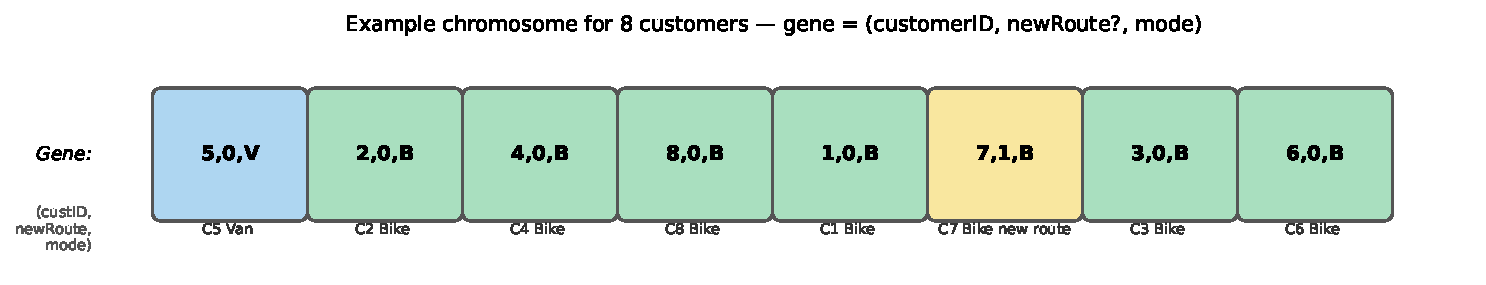
\includegraphics[width=0.90\linewidth]{fig_chromosome.pdf}
  \caption{An example chromosome for 8 customers.
           The first gene places customer 5 on route 1 using a van.
           Gene ``7,1,B'' starts a new route (flag=1) for customer 7
           using a cargo bike.}
\end{figure}

\medskip
\begin{block}{Decoding: from chromosome to routes}
The \textbf{decoder} reads genes left-to-right and builds routes:
\begin{enumerate}
  \item If the new-route flag is 0 and the current customer fits in the
        current route (time window and capacity), append to current route.
  \item If the flag is 1, or the customer does not fit, start a new route.
  \item The \emph{mode} of a route is determined by the first customer's
        mode gene: if that gene says ``V'', the route uses a van; if
        ``B'', the route uses a cargo bike.
\end{enumerate}
\end{block}

\framebreak

\textbf{Worked decoding example.}
Given the chromosome \texttt{5,0,V | 2,0,B | 4,0,B | 8,0,B | 1,0,B | 7,1,B | 3,0,B | 6,0,B}
and the following customer data (time windows, travel times in format
\emph{van}/\emph{bike}):

\medskip
\begin{enumerate}
  \item \textbf{Gene 1 (5,0,V)}: Start route 1 using a van.
        Customer 5 has time window 12:00--13:00.
        Initial arrival time 08:38 (based on depot travel time),
        but window opens at 12:00, so the van waits and arrives at 12:00.
        Routes so far: \quad Route~1V: [5@12:00]

  \item \textbf{Gene 2 (2,0,B)}: Customer 2 has time window 09:00--10:00.
        The earliest arrival from customer 5 at 12:05 is after 10:00
        (the window closes at 10:00), so customer 2 cannot join route 1.
        Because customer 2's mode gene is ``B'', a new bike route is
        started: Route~2B: [2@09:00].

  \item \textbf{Gene 3 (4,0,B)}: Customer 4's window is 13:00--14:00.
        It fits on route 2B after customer 2.
        Route~2B: [2@09:00, 4@13:00].

  \item \textbf{Gene 4 (8,0,B)}: Route 2B is now at capacity (20 units
        for a bike).
        The bike returns to the depot (arriving 13:40), reloads (15 min),
        departs 13:50.
        Customer 8 is added to a new sub-run of route 2B: [2@09:00,
        4@13:00, D, 8@14:01].

  \item \textbf{Gene 5 (1,0,B)}: Customer 1 has window 09:00--10:00.
        Earliest arrival is after 10:00, so a new van route is started.
        This continues until the full chromosome is decoded.
\end{enumerate}

The resulting routes are then evaluated using the cost model to
produce the fitness value $f$ (total distance) and all nine
solution characteristics.

\end{frame}

% ────────────────────────────────────────────────────────────
\begin{frame}[allowframebreaks]{6.3 Setting Archive Boundaries: FindBoundaries}
% ────────────────────────────────────────────────────────────

Before MAP-Elites can scale characteristics into bin indices, it needs
to know the \emph{range} of each characteristic: what are the minimum
and maximum plausible values?
For some characteristics (like the fraction of deliveries by bike),
the range is obvious: [0, 1].
For others (like total staff cost), the range depends on the specific
problem instance and is not known in advance.

\medskip
\begin{block}{Algorithm 15: FindBoundaries}
\textbf{Method 1 (optimise each objective separately):}
\begin{enumerate}
  \item For each characteristic $o$:
        run a separate EA to \emph{optimise} (minimise/maximise) $o$.
  \item Use the resulting population to update the known range of $o$.
\end{enumerate}
\textbf{Method 2 (scan a set of solutions):}
\begin{enumerate}
  \item For each solution in the set:
  \item For each characteristic $o$:
        if solution's value for $o$ is less than known lower bound,
        update lower bound.
        If greater than known upper bound, update upper bound.
\end{enumerate}
\end{block}

\medskip
\begin{block}{Notation}
\begin{itemize}
  \item $objective.lower$ and $objective.upper$: the current known
        minimum and maximum for that characteristic.
  \item These bounds determine $min$ and $max$ in the bin-scaling
        formula, so getting them right is critical for archive quality.
\end{itemize}
\end{block}

\framebreak

\textbf{The seeding technique.}
Table 6.3 shows that for characteristics 1--4 (cost-related) and 8--9
(vehicle counts), the upper bounds are marked ``?'' because they
cannot be determined analytically from an unsolved instance.
The \textbf{seeding} technique addresses this: run 10 independent
short EA runs, collect the final populations, and feed all solutions
into FindBoundaries Method 2.
The EA solutions tend to cover a wide range of the characteristics,
giving realistic bounds.

\medskip
\begin{figure}
  \centering
  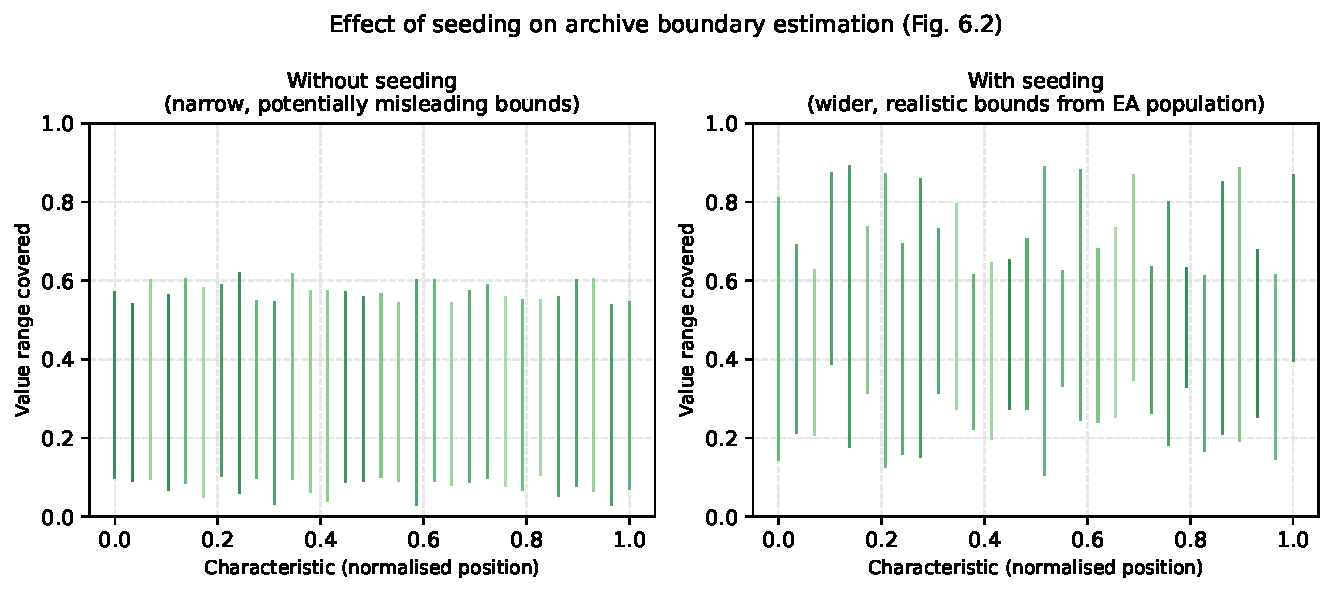
\includegraphics[width=0.80\linewidth]{fig_seeding_effect.pdf}
  \caption{Schematic illustration of the seeding effect.
           Without seeding (left), the archive has narrow, possibly
           misleading bounds.
           With seeding (right), the bounds are wider and more
           realistic, allowing the archive to represent the true
           diversity of the solution space.}
\end{figure}

\framebreak

\begin{alertblock}{Why seeding matters}
If the bounds are set too tight, good solutions outside the range
will be \emph{clipped} to the boundary bins.
Multiple solutions collapse into the same boundary cells, reducing
diversity.
If bounds are set too wide, the bins are very coarse and many
qualitatively different solutions map to the same cell---again
reducing diversity.
Seeding gives a data-driven estimate of realistic bounds from
actual solutions, striking the right balance.
\end{alertblock}

\medskip
The actual parameter ranges found by seeding for the supermarket
delivery problem are shown in the book (Table 6.4).
For example, for \textbf{CostDel} (cost per delivery):
\begin{itemize}
  \item Seeded: lower = 1.18, upper = 11.9 $\Rightarrow$ $\delta \approx 10.72$, bin size $\approx 1.072$
  \item Unseeded: lower = 0, upper = 7.65 $\Rightarrow$ $\delta = 7.65$, bin size $\approx 0.765$
\end{itemize}
The seeded range is about 40\% wider, meaning the archive covers
a broader region of the cost-per-delivery axis.

\end{frame}

% ────────────────────────────────────────────────────────────
\begin{frame}[fragile]{6.3 Java Implementation: The MAP-Elites Solver (Listing 6.1)}
% ────────────────────────────────────────────────────────────

The book provides a Java implementation of MAP-Elites.
The core \texttt{solve()} method is shown below.
Key classes: \texttt{Archive} (sparse hash map of elite solutions),
\texttt{EliteSolution} (extends the EA's individual class with
fitness/key methods), \texttt{EliteSolutionFactory} (creates new
solutions by recombination or cloning).

\medskip
\begin{lstlisting}[language=Java, caption={Listing 6.1: The MapElites algorithm (Java)}]
public void solve() {
    archive = new Archive(KeyGenerator.getInstance().getDimensions(),
                          KeyGenerator.getInstance().getBuckets());
    initialise();
    EliteSolution ch;
    for (int c=0; c < MAX_EVALS; c++) {
        if ((c%10000)==0) {
            System.out.print(" "+c+" : "+ archive.size());
        }
        if (rnd.getRnd().nextBoolean()) {
            // Select two random parents from the archive
            EliteSolution p1 = (EliteSolution)archive.getRandom();
            EliteSolution p2 = (EliteSolution)archive.getRandom();
            // Create a new solution from the parents (crossover)
            ch = (EliteSolution) solutionFactory.getChild(theProblem, p1, p2);
            if (rnd.getRnd().nextBoolean()) {
                ch.mutate();        // Mutate the child solution
            }
        } else {
            // Create a new solution by copying an existing archive member
            ch = solutionFactory.copy((EliteSolution)archive.getRandom());
            ch.evaluate();
            ch.mutate();
        }
        ch.evaluate();
        if (archive.put(ch)) {  // Put into archive; returns true if added
            Logger.getLogger().add(action, descForLogger,
                                   ch.getFitness(), ch.getSummary(), ch.getKey());
        }
    }
    System.out.println();
}
\end{lstlisting}

\medskip
\textbf{Line-by-line explanation:}
\begin{itemize}
  \item Lines 1--3: construct the \texttt{Archive} with the correct
        number of dimensions and bucket sizes from \texttt{KeyGenerator}.
  \item Lines 5--6: print progress every 10,000 evaluations.
  \item Lines 7--15: with 50\% probability, perform \textbf{crossover}:
        select two random parents from the archive, create a child from
        them, optionally mutate.
  \item Lines 16--21: otherwise, \textbf{clone} a random archive member
        and mutate.
  \item Lines 22--24: evaluate the candidate and attempt to add it to
        the archive.  If \texttt{archive.put(ch)} returns \texttt{true},
        the candidate improved upon (or filled) a cell; log it.
\end{itemize}

\end{frame}

% ────────────────────────────────────────────────────────────
\begin{frame}[allowframebreaks]{6.3 Python Equivalent: MAP-Elites Core Logic}
% ────────────────────────────────────────────────────────────

Below is a Python implementation of the MAP-Elites core logic,
demonstrating the same ideas as the Java listing with a simpler
delivery toy problem.
This Python version is self-contained and can be run directly.

\end{frame}

\begin{frame}[fragile]{Python: MAP-Elites Core (Part 1 --- Scaling and Archive)}

\begin{lstlisting}[style=python, caption={Python: bin scaling and archive add}]
import math, random

def scale_to_bin(r, rmin, rmax, b=10):
    """Map raw value r in [rmin, rmax] to bin index 1..b."""
    delta = (rmax + 1) - rmin
    cap   = delta / b
    s     = int((r - rmin) / cap + 1)
    return max(1, min(b, s))   # clamp to valid range

def get_key(solution, descriptors, bounds, b=10):
    """
    Compute the archive key (tuple of bin indices) for a solution.
    solution   : dict of characteristic name -> value
    descriptors: list of characteristic names to use as archive axes
    bounds     : dict of name -> (rmin, rmax)
    """
    key = tuple(
        scale_to_bin(solution[name], bounds[name][0], bounds[name][1], b)
        for name in descriptors
    )
    return key

def archive_add(archive, solution, key):
    """
    Add solution to the archive at position key.
    Returns True if the archive was updated (cell improved or filled).
    Lower fitness is better.
    """
    if key not in archive or solution['fitness'] < archive[key]['fitness']:
        archive[key] = solution
        return True
    return False
\end{lstlisting}

\end{frame}

\begin{frame}[fragile]{Python: MAP-Elites Core (Part 2 --- Main Loop)}

\begin{lstlisting}[style=python, caption={Python: MAP-Elites main loop}]
def map_elites(problem, tot_evals=50_000, xover_pressure=0.5, b=10):
    """
    Run MAP-Elites on 'problem'.
    problem must provide: random_solution(), mutate(sol),
    crossover(sol1, sol2), evaluate(sol), descriptors, bounds.
    Returns the archive (dict: key -> solution).
    """
    archive = {}

    # --- Initialisation phase: 100 random solutions ---
    for _ in range(100):
        sol = problem.random_solution()
        problem.evaluate(sol)
        key = get_key(sol, problem.descriptors, problem.bounds, b)
        archive_add(archive, sol, key)

    # --- Main search loop ---
    for ev in range(100, tot_evals):
        if random.random() < xover_pressure:
            # Crossover: combine two random archive members
            p1 = random.choice(list(archive.values()))
            p2 = random.choice(list(archive.values()))
            child = problem.crossover(p1, p2)
        else:
            # Clone + mutate a random archive member
            child = dict(random.choice(list(archive.values())))

        child = problem.mutate(child)
        problem.evaluate(child)
        key = get_key(child, problem.descriptors, problem.bounds, b)
        archive_add(archive, child, key)

        if (ev % 10_000) == 0:
            print(f"  eval={ev:,}  archive size={len(archive)}")

    return archive

# Example usage (toy delivery problem):
# arch = map_elites(MyDeliveryProblem(), tot_evals=200_000)
# print(f"Final archive: {len(arch)} cells occupied")
# best_low_emit = min(
#     (sol for sol in arch.values() if sol['emissions'] < 50),
#     key=lambda s: s['cost']
# )
\end{lstlisting}

\end{frame}

% ============================================================
\section{6.4 Results}
% ============================================================

\begin{frame}[allowframebreaks]{6.4 Results: Experimental Setup}
% ────────────────────────────────────────────────────────────

The MAP-Elites algorithm was evaluated on the \textbf{Augerat benchmark
instances}: three sets (A, B, P) of vehicle routing problems with
time windows, ranging from small (12 customers) to large (101
customers).
Each problem was solved 10 times independently to obtain reliable
statistics.

\medskip
\begin{block}{Experimental setup}
\begin{itemize}
  \item \textbf{Problem instances}: Augerat sets A (27 problems),
        B (24 problems), P (24 problems) with time windows.
  \item \textbf{Algorithm}: MAP-Elites with $b=10$ bins,
        9 characteristics, sparse hash-map archive.
  \item \textbf{Comparison}: Seeded vs.\ unseeded boundary estimation.
  \item \textbf{Metrics}: archive size (number of occupied cells),
        best fitness found per run, number of feasible solutions.
  \item \textbf{Scenarios}: A1--A4 (aspirations applied to filter the
        archive), C1--C3 (constraints applied), and combinations.
\end{itemize}
\end{block}

\medskip
\textbf{The costing model} assigns a total cost per solution:
\begin{itemize}
  \item Fixed cost per vehicle per day (van: \pounds164, bike: \pounds16).
  \item Running cost per km (van: \pounds0.117, bike: \pounds0.01).
  \item Staff cost at \pounds12/hour for all travel and loading time.
  \item Loading time at 30 min (van) or 15 min (bike) between runs.
\end{itemize}
The fitness value $f$ used within MAP-Elites is the total distance
(in km), which is a good proxy for overall cost and is computationally
cheap to compute.
The nine solution characteristics are derived from $f$ and the
routing details.

\end{frame}

% ────────────────────────────────────────────────────────────
\begin{frame}[allowframebreaks]{6.4 Results: Archive Coverage}
% ────────────────────────────────────────────────────────────

\textbf{Archive coverage} measures how many cells in the archive
contain at least one elite solution.
High coverage means MAP-Elites has found solutions representing a
wide variety of trade-offs.
Low coverage means the algorithm has not fully explored the behaviour
space.

\medskip
\begin{figure}
  \centering
  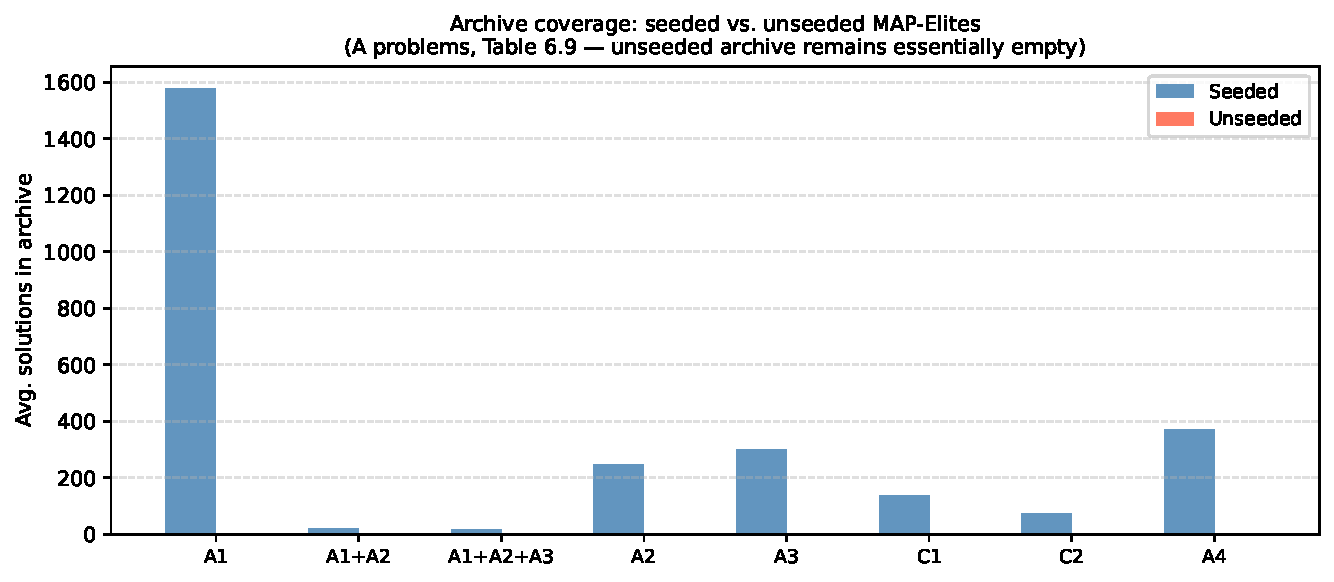
\includegraphics[width=0.75\linewidth]{fig_coverage_bar.pdf}
  \caption{Average archive coverage (number of solutions in the archive)
           for seeded vs.\ unseeded MAP-Elites across selected
           scenarios (A problems, Table 6.9).
           Seeding consistently produces archives with many more
           solutions; unseeded archives remain nearly empty.}
\end{figure}

\framebreak

\begin{block}{Key finding: Seeding is essential}
Table 6.9 in the book shows that when no constraints or aspirations
are applied (scenario A1, meaning ``only aspiration 1 is active''),
the seeded MAP-Elites finds an average of 1{,}576.7 solutions per
problem instance for A problems, while the unseeded version finds
essentially zero.
The seeded version also dominates in terms of ``seeded wins'' (the
seeded archive contains a strictly better solution than the unseeded
archive in almost every problem).
\end{block}

\medskip
\textbf{Why does unseeded fail so completely?}
Without seeding, the archive uses tight, possibly incorrect bounds.
Solutions that the EA generates may map to boundary cells (because
their characteristic values fall outside the unseeded range), causing
many solutions to compete for the same few cells.
The effective archive becomes very small, the algorithm degenerates
into a standard single-population EA, and diversity collapses.

\medskip
\begin{alertblock}{Key Insight: The boundary estimation determines archive quality}
The quality of a MAP-Elites run depends critically on how well the
archive boundaries are set.
Seeding uses actual evolutionary algorithm solutions to set realistic
bounds, and this alone transforms the algorithm from ineffective to
highly effective.
This is a practical lesson: \emph{always} seed your MAP-Elites
boundaries from domain knowledge or preliminary runs.
\end{alertblock}

\end{frame}

% ────────────────────────────────────────────────────────────
\begin{frame}[allowframebreaks]{6.4 Results: Constraints and Aspirations}
% ────────────────────────────────────────────────────────────

One of the most powerful features of the MAP-Elites archive is that
a manager can \textbf{interactively filter} it in real time by applying
\textbf{constraints} and \textbf{aspirations}, without re-running
the algorithm.

\medskip
\begin{block}{Constraints (C): hard limits}
A constraint removes from consideration any solution that violates a
hard limit.
\begin{itemize}
  \item \textbf{C1 --- Vehicle shortage}: only 2 vans can be operated
        on this day (e.g., due to maintenance).
        Remove all archive solutions that use more than 2 vans.
  \item \textbf{C2 --- Cargo bike shortage}: only 2 cargo bikes are
        available.
        Remove all archive solutions requiring more than 2 bikes.
  \item \textbf{C3 --- Emissions cap}: a regulatory or corporate
        emissions ceiling applies.
        Remove all solutions exceeding the cap.
\end{itemize}
Constraints are applied as filters over the archive and do not change
the archive itself---the removed solutions remain available and can be
restored if the constraint is relaxed.
\end{block}

\medskip
\begin{block}{Aspirations (A): soft preferences}
An aspiration is a preference to move in a certain direction in the
solution space.
\begin{itemize}
  \item \textbf{A1}: Reduce staff cost and running cost
        (minimise operational expenditure).
  \item \textbf{A2}: Maximise the fraction of deliveries made by cargo
        bike (sustainability preference).
  \item \textbf{A3}: Reduce fixed vehicle costs (use fewer or cheaper
        vehicles).
  \item \textbf{A4}: Minimise cost per delivery unit.
\end{itemize}
Aspirations are applied by restricting the axis ranges in the archive,
effectively zooming in to the region of the archive that meets the
aspiration.
\end{block}

\framebreak

\textbf{Interactive filtering workflow.}
\begin{enumerate}
  \item Run MAP-Elites once to produce the full archive (may take minutes
        to hours depending on problem size).
  \item Present the archive to the manager as a parallel coordinates
        plot, with each axis corresponding to one characteristic.
  \item The manager applies a constraint (e.g., ``I only have 2 vans
        today''):
        all solutions with more than 2 vans are greyed out.
  \item The manager adds an aspiration (e.g., ``I want to minimise
        running cost''): the archive is filtered to show only
        solutions below a running-cost threshold.
  \item The manager browses the remaining solutions and selects one.
\end{enumerate}
This interactive process happens in \textbf{seconds}, because it is
just filtering a pre-built data structure.

\medskip
\begin{figure}
  \centering
  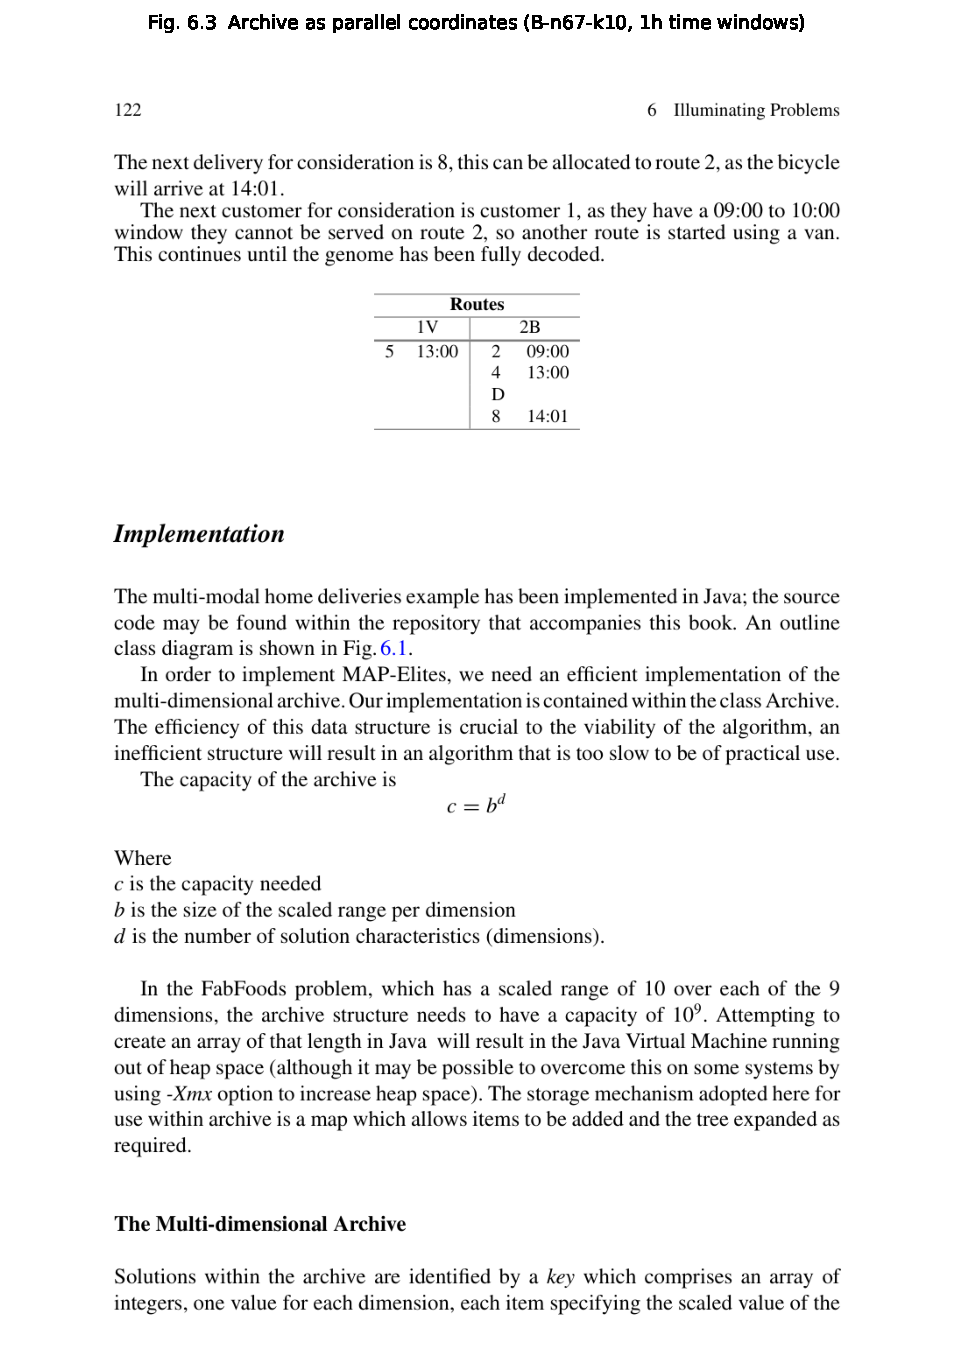
\includegraphics[width=0.88\linewidth]{fig_book_fig6_3.pdf}
  \caption{Fig.\ 6.3 from the book: the MAP-Elites archive for
           problem B-n67-k10 with 1-hour time windows, shown as a
           parallel coordinates plot.
           (a) Full archive with no filters.
           (b) After applying constraint C2 (vehicle shortage: at most
           2 vans).
           (c) After applying C2 and aspiration A2 (reduce staff and
           running costs).
           Observe how each filter progressively narrows the
           solution set.}
\end{figure}

\framebreak

\textbf{Quantitative results (Table 6.8, selected scenarios).}
The table below summarises the average number of solutions left in the
archive after applying scenarios to A-problems over 10 runs.
Seeded archives consistently produce more choices under every scenario.

\medskip
\begin{center}
\renewcommand{\arraystretch}{1.2}
\begin{tabular}{lcc}
\toprule
Scenario & Seeded (avg.\ sols) & Unseeded (avg.\ sols) \\
\midrule
A2 A3 (no constraint)         & 15.2 & 0 \\
A1 A2                         & 19.4 & 0 \\
A1 (single aspiration)        & 1576.7 & 0 \\
A2                            & 248.6  & 0 \\
C1 (vehicle constraint only)  & 137.8  & 0 \\
\bottomrule
\end{tabular}
\end{center}

\medskip
\begin{alertblock}{Key Insight: Aspirations reduce but do not eliminate choices}
Applying more aspirations reduces the number of solutions in the archive
(from 1576 to 15 in the most restrictive case), but the seeded archive
\emph{always} provides at least some solutions for the manager to
choose from.
The unseeded archive provides none.
This is the practical payoff of quality-diversity: a rich archive
remains useful even after heavy filtering.
\end{alertblock}

\end{frame}

% ────────────────────────────────────────────────────────────
\begin{frame}[allowframebreaks]{6.4 Results: Parallel Coordinates Visualisation}
% ────────────────────────────────────────────────────────────

\textbf{Parallel coordinates plots} provide a way to visualise and
interact with the high-dimensional archive.
Each vertical axis represents one solution characteristic.
Each horizontal polyline (connecting all axes) represents one elite
solution in the archive.
A manager can ``brush'' an axis (restrict its range) to filter
solutions interactively.

\medskip
\begin{figure}
  \centering
  
\includegraphics[width=0.88\linewidth]{fig_parallel_coords.pdf}
  \caption{Illustrative parallel coordinates plot of an elite archive
           with 9 characteristics.
           Each green line represents one elite solution.
           Darker green lines correspond to solutions with lower
           fixed cost.
           The highlighted blue line is an example selected solution
           with low emissions (axis 5 near 0) and high bike usage
           (axes 6--7 near top).}
\end{figure}

\medskip
\begin{block}{How to read a parallel coordinates plot}
\begin{itemize}
  \item Each \textbf{vertical axis} represents one characteristic.
        Values increase from bottom to top.
  \item Each \textbf{line} (polyline) is one solution.
        A line that stays low on the ``Emissions'' axis and high on
        the ``\%Cycle Deliveries'' axis represents a predominantly
        bike-based, low-emission plan.
  \item \textbf{Crossings} between lines near an axis indicate that
        two solutions have very different values for that characteristic
        but converge elsewhere---they represent qualitatively different
        plans with similar overall cost.
  \item \textbf{Brushing} (restricting the range of an axis) is the
        interactive filtering operation: it corresponds to applying a
        constraint or aspiration.
\end{itemize}
\end{block}

\end{frame}

% ────────────────────────────────────────────────────────────
\begin{frame}[allowframebreaks]{6.4 Results: Summary Tables (A, B, P Problems)}
% ────────────────────────────────────────────────────────────

The results across all three benchmark sets (A, B, P problems from
Tables 6.5--6.7) show consistent patterns:

\medskip
\begin{block}{Summary findings from Tables 6.5--6.7}
\begin{itemize}
  \item \textbf{Fitness quality}: the seeded and unseeded versions
        produce similar \emph{best fitness} values when they do find
        solutions.
        The primary advantage of seeding is in archive \emph{coverage}
        (how many cells are filled), not in the quality of individual
        solutions.
  \item \textbf{Problem scaling}: larger problems (more customers)
        generally produce larger archives, because there is more
        solution diversity possible.
        Problem P-n101-k4-1 (101 customers, 4 vehicles) produces some
        of the largest archives.
  \item \textbf{Bike usage in unseeded results}: interestingly, in
        all presented results, the percentage of cycle deliveries
        and cycle distance is 0/0 in both seeded and unseeded runs.
        This suggests that under the cost model, cargo bikes are rarely
        chosen by the EA as the default mode, and the MAP-Elites
        archive in the main runs focuses primarily on van-based plans.
        The seeding and archive structure allow the \emph{presence}
        of bike solutions, but the fitness function (total distance)
        may not sufficiently incentivise bike usage.
\end{itemize}
\end{block}

\medskip
\begin{exampleblock}{Example from Table 6.5 (A problems, selected rows)}
For problem A-n32-k5-1 (32 customers, 5 vehicles):
\begin{itemize}
  \item Archive size: 5047 total solutions, average fitness 5285.5
        (seeded), 5179.1 (unseeded).
  \item Fixed cost: \pounds288 (seeded run) to \pounds304 (unseeded).
  \item Staff cost: \pounds181--\pounds142.6, running cost: \pounds46--\pounds59.
  \item Cost per delivery: \pounds2.29--\pounds2.28 per unit.
\end{itemize}
This shows the range of costs across the 10 independent runs,
illustrating the natural variability in the evolutionary process.
\end{exampleblock}

\end{frame}

% ============================================================
\section{6.5 Conclusions}
% ============================================================

\begin{frame}[allowframebreaks]{6.5 Conclusions}
% ────────────────────────────────────────────────────────────

This chapter has demonstrated how \textbf{MAP-Elites}, an illumination
algorithm from the Quality-Diversity family, can be applied to the
multi-mode supermarket delivery problem to produce a rich, browsable
archive of high-quality delivery plans.

\medskip
\begin{block}{What MAP-Elites achieves}
\begin{itemize}
  \item It produces a \textbf{structured collection} of diverse plans
        rather than a single solution, giving the operations manager
        genuine choice.
  \item The archive can be \textbf{filtered interactively} (in seconds)
        by applying constraints (hard operational limits) and aspirations
        (soft preferences), without re-running the algorithm.
  \item When properly seeded, the archive provides meaningful choices
        even under multiple simultaneous constraints.
\end{itemize}
\end{block}

\medskip
\begin{block}{Design lessons}
\begin{enumerate}
  \item \textbf{Seed the boundaries}: always use a preliminary
        evolutionary run (seeding) to estimate archive bounds.
        Unseeded archives remain nearly empty, defeating the purpose
        of MAP-Elites.
  \item \textbf{Choose behaviour descriptors carefully}: the nine
        characteristics used here were selected to cover the key
        concerns of all stakeholders (financial, operational,
        environmental).
        Choosing irrelevant characteristics wastes archive capacity
        and increases computational cost.
  \item \textbf{Sparse storage is essential} for high-dimensional
        archives (9 dimensions with $b=10$ gives $10^9$ possible
        cells; a dense array would require terabytes).
        A hash map that only stores occupied cells scales gracefully.
  \item \textbf{The fitness function and descriptors are decoupled}:
        the fitness (total distance) drives within-cell competition;
        the descriptors (9 characteristics) define which cell.
        This decoupling is a deliberate and powerful design choice.
\end{enumerate}
\end{block}

\framebreak

\begin{alertblock}{Key Insight: Illumination vs.\ optimisation}
Classical optimisation asks: ``What is the best solution?''
MAP-Elites asks: ``What is the best solution \emph{for each type of
behaviour}?''
By answering the second question, MAP-Elites gives the decision-maker
far more information and flexibility.
The algorithm \emph{illuminates} the problem by showing what is
achievable across the full behaviour space, not just at one point.
\end{alertblock}

\medskip
\textbf{Limitations and future directions.}
\begin{itemize}
  \item The current results show that cargo bikes are rarely selected
        under the default fitness function (total distance).
        Future work could use a multi-objective fitness or an explicit
        bonus for bike usage.
  \item The archive building phase (MAP-Elites search) is still
        computationally expensive for very large instances.
        Parallel evaluation of candidates could reduce wall-clock time.
  \item The 9-dimensional archive with $b=10$ bins gives $10^9$
        theoretical cells; only a tiny fraction are ever filled.
        Adaptive binning (varying $b$ by dimension based on solution
        density) could improve coverage efficiency.
\end{itemize}

\medskip
\begin{block}{Chapter 6 in one sentence}
MAP-Elites illuminates the delivery planning problem by building a
sparse archive of elite solutions covering every region of the
nine-dimensional behaviour space, enabling real-time interactive
selection by the operations manager.
\end{block}

\end{frame}

% ============================================================
\section{Algorithm Reference}
% ============================================================

\begin{frame}[allowframebreaks]{Algorithm Summary: MAP-Elites (Algorithm 14)}

\begin{block}{Complete pseudocode}
\begin{enumerate}
  \item[] \textbf{Procedure} MAP-Elites(init, totEvals, xOverPressure)
  \item $buckets \leftarrow 20$; \quad $dimensions \leftarrow 2$; \quad $evals \leftarrow 0$
  \item $map$.initialise($buckets$, $dimensions$)
  \item[] \textbf{while} $evals < init$ \textbf{do}
  \item \quad $n \leftarrow$ newIndividual()
  \item \quad $evals \mathrel{+}= 1$
  \item \quad add($map$, $n$)
  \item[] \textbf{while} $evals < totEvals$ \textbf{do}
  \item \quad \textbf{if} random() $<$ xOverPressure \textbf{then}
  \item \quad\quad $c \leftarrow$ newIndividual($map$.random(), $map$.random())
  \item \quad \textbf{else}
  \item \quad\quad $c \leftarrow$ newIndividual($map$.random())
  \item \quad $c$.mutate()
  \item \quad add($map$, $c$)
  \item[] \textbf{return} $map$
  \item[] \textbf{Procedure} add($map$, $n$)
  \item $key \leftarrow$ getKey($n$)
  \item \textbf{if} $map$.get($key$) == null \textbf{then}
  \item \quad $map$.put($key$, $n$)
  \item \textbf{else}
  \item \quad $old \leftarrow map$.get($key$)
  \item \quad \textbf{if} new.fitness() $<$ old.fitness() \textbf{then}
  \item \quad\quad $map$.put($key$, $n$)
  \item[] \textbf{EndProcedure}
\end{enumerate}
\end{block}

\end{frame}

% ────────────────────────────────────────────────────────────
\begin{frame}[allowframebreaks]{Algorithm Summary: FindBoundaries (Algorithm 15)}
% ────────────────────────────────────────────────────────────

\begin{block}{Complete pseudocode}
\begin{enumerate}
  \item[] \textbf{Procedure} findBoundaries($problem$, $objectives$)
  \item \textbf{for each} Objective $o$ in $objectives$ \textbf{do}
  \item \quad $sols \leftarrow$ optimise($o$, $prob$)
  \item \quad updateRanges($sols$)
  \item[] \textbf{EndProcedure}
  \item[]
  \item[] \textbf{Procedure} findBoundaries($solutions$)
  \item \textbf{for each} Solution $sol$ in $solutions$ \textbf{do}
  \item \quad \textbf{for each} Objective $obj$ in $objectives$ \textbf{do}
  \item \quad\quad \textbf{if} $sol[obj].lower < obj.lower$ \textbf{then}
  \item \quad\quad\quad $obj.lower \leftarrow sol[obj].lower$
  \item \quad\quad \textbf{if} $sol[obj].upper > obj.upper$ \textbf{then}
  \item \quad\quad\quad $obj.upper \leftarrow sol[obj].upper$
  \item[] \textbf{EndProcedure}
\end{enumerate}
\end{block}

\medskip
\begin{block}{Notation}
\begin{itemize}
  \item $obj.lower$, $obj.upper$: the running minimum and maximum
        values seen so far for characteristic $obj$.
        These bounds are used as $min$ and $max$ in the bin-scaling
        formula.
  \item \texttt{optimise($o$, $prob$)}: run a single-objective EA
        to minimise/maximise characteristic $o$ on problem $prob$.
        Returns a set of solutions.
  \item \texttt{updateRanges($sols$)}: scan all solutions in $sols$
        and update bounds (same as Method 2 above).
\end{itemize}
\end{block}

\end{frame}

% ============================================================
\section{Worked Examples}
% ============================================================

\begin{frame}[allowframebreaks]{Worked Example: Full MAP-Elites Run (2D Archive)}

This worked example traces through a miniature MAP-Elites run with
2 characteristics ($c$ = cost, $e$ = emissions), $b=5$ bins each
(25 cells), and only 10 candidate solutions for clarity.

\medskip
\begin{block}{Setup}
$c \in [400, 700]$: $\delta = 301$, $cap = 60.2$, bins 1--5 \\
$e \in [900, 1200]$: $\delta = 301$, $cap = 60.2$, bins 1--5
\end{block}

\medskip
\begin{exampleblock}{Candidate solutions and their bin keys}
\begin{center}
\renewcommand{\arraystretch}{1.2}
\begin{tabular}{ccccccc}
\toprule
Sol & $c$ & $e$ & $f$ (dist) & $s_c$ & $s_e$ & Key \\
\midrule
1 & 450 & 950  & 320 & 1 & 1 & (1,1) \\
2 & 520 & 980  & 290 & 2 & 2 & (2,2) \\
3 & 610 & 1050 & 340 & 4 & 3 & (4,3) \\
4 & 460 & 960  & 310 & 1 & 1 & (1,1) --- collision \\
5 & 680 & 1150 & 280 & 5 & 5 & (5,5) \\
6 & 460 & 960  & 330 & 1 & 1 & (1,1) --- collision \\
7 & 530 & 1100 & 295 & 2 & 4 & (2,4) \\
8 & 590 & 1000 & 305 & 4 & 2 & (4,2) \\
\bottomrule
\end{tabular}
\end{center}
\end{exampleblock}

\medskip
\textbf{Step-by-step archive updates:}
\begin{itemize}
  \item Sol 1 arrives at (1,1): cell empty $\Rightarrow$ place. $f[(1,1)]=320$.
  \item Sol 2 arrives at (2,2): empty $\Rightarrow$ place. $f[(2,2)]=290$.
  \item Sol 3 arrives at (4,3): empty $\Rightarrow$ place. $f[(4,3)]=340$.
  \item Sol 4 arrives at (1,1): occupied. $310 < 320$ $\Rightarrow$ \textbf{replace}. $f[(1,1)]=310$.
  \item Sol 5 arrives at (5,5): empty $\Rightarrow$ place. $f[(5,5)]=280$.
  \item Sol 6 arrives at (1,1): occupied. $330 > 310$ $\Rightarrow$ \textbf{rejected}.
  \item Sol 7 arrives at (2,4): empty $\Rightarrow$ place. $f[(2,4)]=295$.
  \item Sol 8 arrives at (4,2): empty $\Rightarrow$ place. $f[(4,2)]=305$.
\end{itemize}

\medskip
\textbf{Final archive}: 6 cells occupied out of 25.
Cell (1,1) holds solution 4 (lower cost, lower emissions, shorter
routes than solution 1).
Solution 6 was rejected despite having the same cell as solutions 1
and 4, because its distance (330 km) was worse than the current
occupant (310 km).

\end{frame}

% ============================================================
\section{References}
% ============================================================

\begin{frame}{References}
\begin{itemize}
  \item Mouret, J.-B. \& Clune, J. (2015).
        \emph{Illuminating Search Spaces by Mapping Elites}.
        arXiv:1504.04909.
        [The original MAP-Elites paper; the foundation of this chapter.]

  \item Augerat, P. (1995).
        \emph{Approche poly\'{e}drale du probl\`{e}me de tourn\'{e}es de
        v\'{e}hicules} (Ph.D.\ Thesis, Grenoble Institute of Technology).
        [The benchmark vehicle routing instances used in the experiments.]

  \item Augerat, P. (2014a/b/c).
        VRP-REP: Augerat 1995 Sets A, B, P.
        \url{http://www.vrp-rep.org/datasets/item/2014-0000.html}
        [Online datasets used for experiments.]

  \item Holland, J.\ H. (1975).
        \emph{Adaptation in Natural and Artificial Systems}.
        University of Michigan Press.
        [Foundation of evolutionary algorithms, underlying the EA
        operators used in MAP-Elites.]

  \item Inselberg, A. (2009).
        \emph{Parallel Coordinates: Visual Multidimensional Geometry
        and Its Applications}.
        Springer.
        [The visualisation technique used to present the archive
        interactively.]
\end{itemize}
\end{frame}

% ============================================================
% Summary slide
% ============================================================
\begin{frame}{Chapter 6 Summary}

\begin{block}{Core concepts reviewed}
\begin{tabular}{ll}
\toprule
\textbf{Concept} & \textbf{Key point} \\
\midrule
Quality-Diversity (QD) & Optimise quality AND coverage simultaneously \\
MAP-Elites & Archive of best solution per behaviour region \\
Behaviour descriptors & Solution characteristics defining archive axes \\
Bin-scaling formula & $s = \mathrm{int}\!\left(\frac{r-min}{cap}+1\right)$, $cap = \frac{\delta}{b}$ \\
Archive update rule & Replace cell occupant only if $f_{new} < f_{old}$ \\
Archive capacity & $c = b^d$ (exponential in dimensions, use sparse map) \\
Seeding & Preliminary EA runs set realistic archive bounds \\
Constraints/Aspirations & Interactive post-hoc filtering in seconds \\
\bottomrule
\end{tabular}
\end{block}

\medskip
\begin{alertblock}{The single most important idea in Chapter 6}
MAP-Elites separates the \emph{search phase} (run once, potentially
expensive) from the \emph{decision phase} (run many times, cheap).
The archive is the bridge: built once, queried many times, filtered
interactively to support real-world decision-making under changing
constraints.
\end{alertblock}

\end{frame}

\end{document}
